%!TEX root = thesis.tex

\chapter{Robot simulation}
\label{chap:simulation}

This chapter focuses on the simulation part of the thesis. The objective is the creation of a simulation model, particularly designed for the IIS lab robot setup. The model has to reflect the properties and behaviour of the contained robot components as good as possible. Certainly the simulated components have to provide the same control interface as their real counterparts, allowing to test and optimize control code on the simulator before utilizing it on the real robot. Preferably, the control code sees no difference about on which instance it is executed. The recommendations on such a solution can be summarized as follows: 

\begin{itemize}

\item
The simulator needs to be able to generate realistic sensor and feedback data that can be used by the control software. This includes forces and torques that are measured within force sensors, the current state of the various robot joints (position, velocity, effort), but also RGB and depth images, usually produced by Kinect cameras and vision sensors.

\item
The simulation solution has to provide exactly the same ROS control interface as the real robot. This interface essentially consists of a number of ROS topics, that can be used to send control commands to the various different robot components or to read actual joint states and sensor data.
 
\item
The utilized simulation platform has to provide a graphical user interface that allows to visualize the motions of the robot and it's interaction with the environment. Possibly accidental collisions of  robot parts have to be registered and should also be visualized.

\item
In order to be used by as many people as possible, it is very important that the solution is really easy to use and does not require a long lead time. Therefore it has to be put particular focus on usability.

\end{itemize}

The following sections explain in detail, how this goal was reached. At the beginning stands the process of finding a suitable simulation platform that meets the requirements and the considered criteria. After that, the chosen simulation platform V-Rep is introduced and an overview about how to design dynamic simulations is given, explaining some of the necessary terminology. Subsequent sections focus on the necessary steps to achieve the final solution, namely finding and modelling required robot components, assembling and configuring the final simulation scene and the implementation of the ROS control interface.

\section{Choosing a suitable simulation platform}

The tasks executed on the robot are in most cases variations of so called 'pick and place' tasks. An object gets picked up, lifted and placed somewhere else within the robot's workspace. Therefore joint target positions are sent to the control interfaces of the various robot components and they execute the commanded motions if possible. The question, if the execution is possible at all and in that case in which velocity, is influenced by a number of dynamic parameters. The maximum effort of the motors in the joints is limited. If the force that acts upon a joint is higher than the maximum effort of the motor it will not be able to maintain its current position or to reach the desired target position. This can happen if the picked object is to heavy or if the robot collides with an immovable object in it's environment. The forces that act upon each single joint are influenced by a number of parameters like the position within the kinematic chain of the robot, the summed own weight of the robot components and also the weight of a possibly additional payload.

The required solution should be able to provide a realistic simulation of those dynamic interactions. Therefore the utilized simulation platform has to take use of a powerful physics engine. A physics engine is a software component, that is capable of computing parameters of physical processes and the dynamic properties of the involved objects. Examples for such engines are the Open Dynamics Engine\footnote{http://www.ode.org} (ODE) and Bullet physics\footnote{http://bulletphysics.org}. Some of the evaluated simulation platforms even provide a number of different physics engines to choose.\\

The candidates that have been taken into account were Gazebo\footnote{http://gazebosim.org/}, V-Rep\footnote{http://coppeliarobotics.com}, MORSE\footnote{http://www.openrobots.org/wiki/morse/} and Openrave\footnote{http://openrave.org}. After some investigation only two of them (Gazebo and V-Rep) had been evaluated in greater detail. Criteria for the selection had been:

\begin{itemize}
\item
Which physics engine is used respectively is it possible to choose among various engines?
\item
Usability and stability
\item
Expandability
\item
Availability of required model components (arm model, gripper,...)
\item
Quality of the documentation
\item
Licence issues
\end{itemize}

Taking into account those criteria it went clear that V-Rep will be the simulation platform of choice. In some initial tests V-Rep seemed to be much more stable than Gazebo and the user interface is very intuitive. Another important point is that V-Rep ships with a fully functional model of the KUKA LWR4+ robot arm.

\section{The Virtual Robot Experimentation Platform(V-Rep)}
V-Rep is a powerful robot simulation platform, developed by Coppelia Robotics. The current version (V3.1.2) provides the ability to choose from three configurable physics engines (ODE, Bullet, Vortex -- only trial version) for simulating dynamic processes. It also contains a very comfortable editor for modelling robot components and simulation scenes. In the \emph{shape edit mode} it is possible to edit and simplify meshes. This is very important because for simulating dynamic processes only simple shapes with a low amount of vertices, edges and faces should be used to reduce complexity. The contained model browser provides a rich set of different robot models, static objects and various sensors, ready to use. A powerful feature are V-Rep's so called \emph{calculation modules}. They can be configured to provide additional calculation functionalities on groups of scene objects. The \emph{collision detection module} is capable of detecting and visualizing all kinds of collisions within the simulation scene. The \emph{inverse kinematics calculation module} allows to solve inverse kinematics problems for robot components. The behaviour of the simulator is highly customizable via a rich programming API for C++ as well as the scripting language LUA\footnote{http://www.lua.org}. V-Rep is no open source software but it provides a free licence for educational units and can therefore be used for research purposes. A more detailed introduction to V-Rep can be found in \cite{freese2013}.

\section{Dynamic simulations in V-REP}
For a better understanding of the modelling process it is necessary to explain a few fundamental concepts about designing dynamic simulations in V-Rep. This section just covers those aspects that are important for the underlying project. A more detailed explanation can be found in the official V-Rep documentation\footnote{http://www.coppeliarobotics/helpFiles}. \\

Each simulation scene in V-Rep is composed from a number of models that are arranged within the environment. A model consists of various scene object, combined in a tree like structure to mimic the kinematic chain of a robot component. Each model has a dedicated model base and constitutes a sub-tree of the scene hierarchy. The model base is the root element of the model tree. There are existing various types of scene objects within V-Rep, but only those, which are important for the implementation will be explained here.

\begin{itemize}
\item \textbf{Shape} \\
A shape is a 3 dimensional body. Shapes represent the visual parts as well as the dynamically enabled parts of the scene. It is necessary to distinguish between primitive shapes (Cylinder, Cuboid, Sphere, Plane and Disk) and complex shapes (triangle meshes). Primitive shapes are much easier to handle for the physics engine as there can happen a lot of optimization during dynamics calculations. Complex shapes usually look better and therefore they are used mainly as the visual part of the model but also by the collision detection module. Various shapes can be combined to groups and therefore treated as one single object. Shapes can be defined as \emph{static} or \emph{non-static} objects. The position of a static object is fixed relative to it's parent node within the scene hierarchy and will not change during simulation. Non-static objects underlie gravity and will fall down if they are not constrained by a dynamically enabled joint or a force sensor connection. It is also necessary to distinguish between \emph{respondable} and \emph{non-respondable} shapes. Respondable shapes have a clearly defined mass and moment of inertia and therefore they create collision reactions when colliding with other respondable objects during simulation. Only respondable shapes are considered during dynamics calculation. Usually a model in V-Rep is composed of a visual part, consisting of complex shapes and a hidden part, consisting of groups of primitive shapes that are configured to be used for the dynamics calculations. This issue will be covered again when explaining the creation of the hand model. Each shape also has some additional flags, defining special attributes used by the \emph{calculation modules}. The \emph{collidable} attribute states that a shape has to be considered during collision detection. The \emph{renderable} flag marks a shape to be recognized by a \emph{vision sensor}. There are more flags available but only those two were used within this project.

\item \textbf{Joint} \\
A joint is a flexible connection between two rigid parts of a robot. It has to be distinguished between revolute or prismatic joints with one degree of freedom and spherical joints with three degrees of freedom. In the arm and hand model only revolute joints are used. Joints can be passive or actuated by a motor. The motor settings include maximum force or torque and velocity limits. If the control loop is enabled then a desired target position for the joint can be set. The controller will then try to reach this position, based on it's PID settings while respecting the motor limits. It would also be possible to program a custom control loop for each joint but for the current project this is not necessary. Joints can be operated in various different modes. A joint in \emph{torque/force mode} is simulated, using the physics engine. This is the most realistic control mode. A joint in \emph{inverse kinematics mode} is controlled by the inverse kinematics calculation module and if additionally the option \emph{hybrid operation} is selected then the dynamic parameters of the joint are also taken into account. Operating a joint in \emph{dependent mode} means that it's position depends on the position of another joint within the scene. How this dependency looks like can be configured by setting a \emph{dependency equation}.

\item \textbf{Vision sensor} \\
States a simulated image capturing device. A vision sensor can capture images of the simulation scene, depending on it's configuration. It can deliver RGB image sequences as well as depth images. Vision sensors are used in the Kinect camera model.

\item \textbf{Force sensor} \\
A force sensor in V-Rep is a rigid connection between two dynamically simulated objects. The calculated forces and torques can be measured and visualized. It is also possible to define a maximum force the connection is able to bear. When this maximum value is exceeded, the connection will break.

\item \textbf{Dummy} \\
Dummies are the simplest scene objects at all but they provide some important functionality, especially for the various calculation modules of V-Rep. They can be understood as the origin of a named reference frame with a configurable position and orientation within the simulation scene. Two dummies can be linked as \emph{tip-target pairs} to be used by the IK calculation module. The importance becomes more clear when the construction of the simulation scene will be explained, particularly when configuring the inverse kinematics calculation module. 

\end{itemize}

Groups of scene objects can be organized in \emph{collections} and treated as one single entity. Collections play an important role in the collision detection module.


\section{Designing the simulation scene}
This section explains in detail the structure of the simulation scene and the contained model components. The setup contains three types of robot component - the Kuka LWR4+ robot arm, the Schunk SDH-2 gripper and the Kinect camera. For each one of them, a simulation model was required in order to be able to build up the scene. V-Rep ships with realistic and fully functional model for the Kuka arm and also for the Kinect camera. But as there is currently no model for the Schunk gripper available, it had to be created from scratch. The necessary steps of the modelling process are explained in the next section.

\subsection{Modelling the Schunk SDH-2 gripper}

A model within a V-Rep simulation scene basically consists of three major parts. First there are the shapes that form the visual part of the model. Those shapes are triangle meshes for each single link of the robot component. Preferably they are not to complex, i.e. the amount of faces is not to high. The second part is formed by the joints that connect those shapes and allow to actuate the flexible parts of the model. The third part consists of the dynamically enabled parts of the model. Theese shapes form the body of the model, how it is seen by the physics engine. Those respondable parts are usually an approximation of the original meshes, composed from groups of primitive shapes. Those parts are very important as they make the model realistic and allow to interact with other respondable objects within the scene. Without them, the model would just move through other bodies as only respondable shapes are able to produce collision reactions. The steps, described within this section enclose the modelling of that three parts for the gripper model.\\

\begin{figure}[ht]
	\centering
  	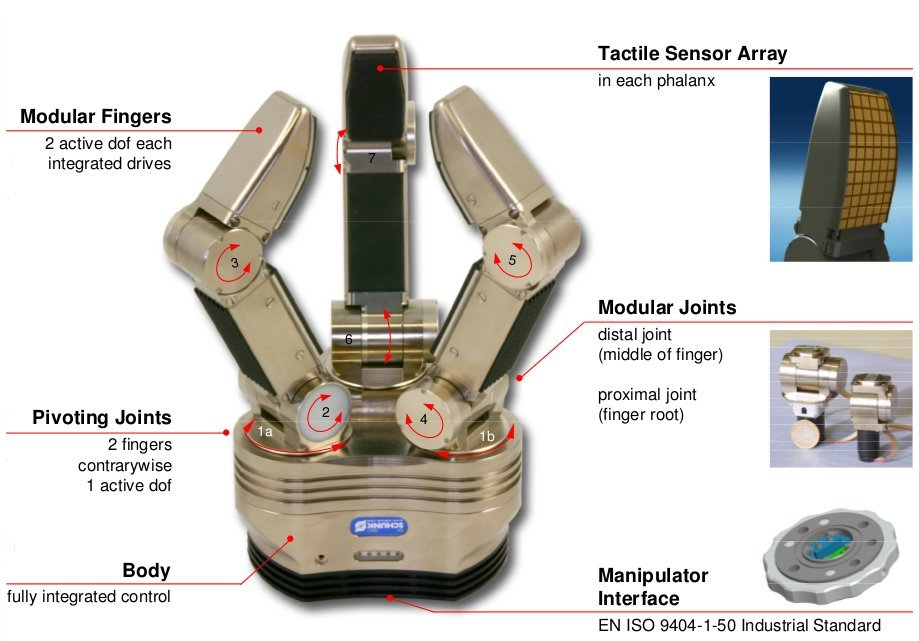
\includegraphics[width=1.0\textwidth]{images/sdh_sheet.jpg}
	\caption[Schunk SDH-2 (source: Schunk data sheet\cite{buss2004})]{Schunk SDH-2 gripper}
	\label{fig:sdh_sheet}
\end{figure}

Figure\ref{fig:sdh_sheet} shows the Schunk SDH-2 hand. The gripper has 3 fingers, each one containing two modular joints. The joints located closer to the wrist are called the \emph{proximal} finger joints whereas the joints, actuating the finger tips are called the \emph{distal} finger joints. Two of the fingers can be rotated along their vertical axis but they are connected contrariwise. That means if one finger rotates to the left, the other one is rotated to the right for the same angle, actually adding one additional degree of freedom. Those two joints are called the \emph{pivoting} joints. The visual part of the hand model basically consists of 4 different shapes - the wrist, finger knuckles, finger links and finger tips. Suitable meshes were taken from the schunk\_description\footnote{http://wiki.ros.org/schunk\_description} ROS package and imported into the V-Rep robot editor. They have then been arranged according to the technical description. The next step was to insert and arrange the gripper joints on their appropriate locations.

\begin{figure}[t]
	\centering
  	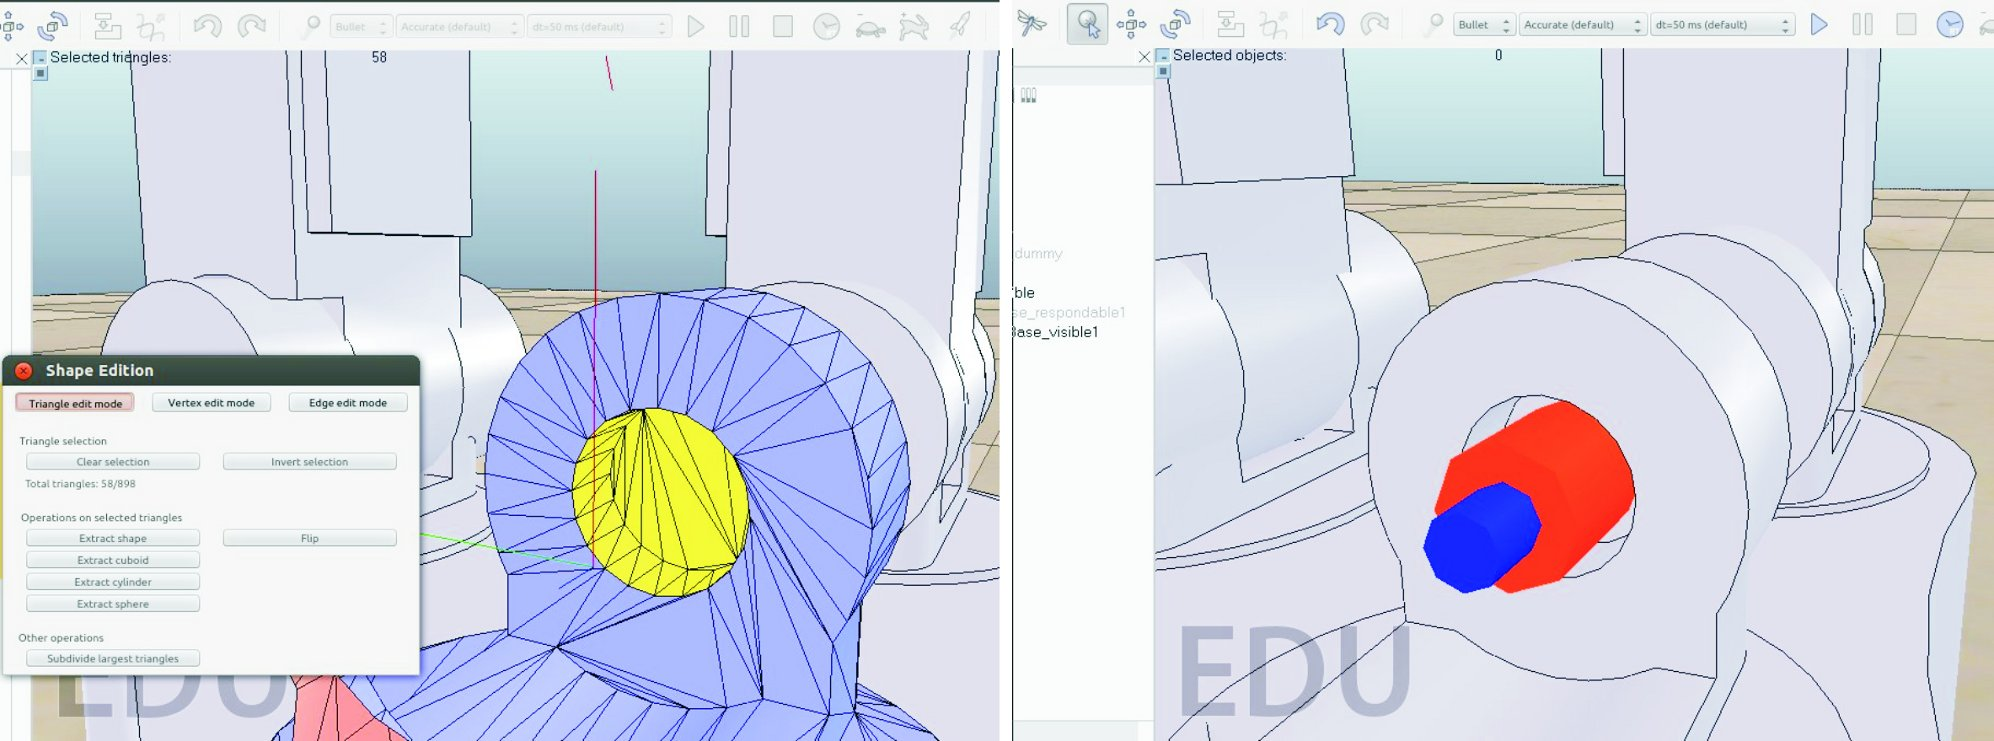
\includegraphics[width=1.0\textwidth]{images/place_joint.jpg}
	\caption{Placing a joint within the model}
	\label{fig:place_jnt}
\end{figure}

Therefore it was important to determine the correct position and orientation for each single joint within the model to allow the correct movement of the fingers. This was achieved by using the \emph{shape edit mode} and select the cylinder shaped area within the mesh, where the joint has to fit. From that selection a cylinder was extracted and the joint was then centred within this newly created cylinder. Those steps had to be repeated for all 8 joints. The placement process can be seen in Figure\ref{fig:place_jnt}.

\begin{figure}[b]
	\centering
  	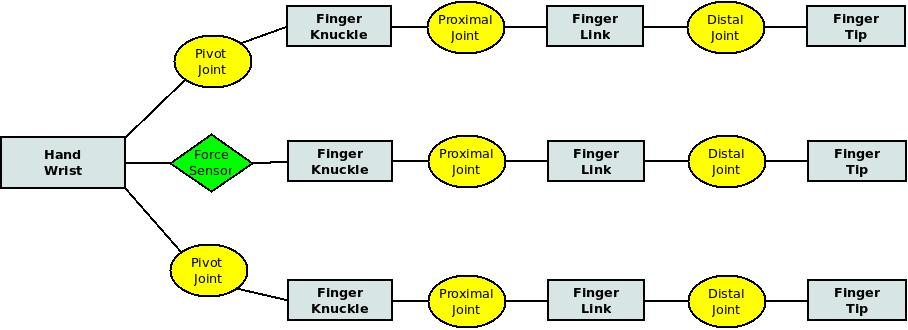
\includegraphics[width=1.0\textwidth]{images/hand_tree.jpg}
	\caption{Kinematic chain of the Schunk gripper}
	\label{fig:hand_tree}
\end{figure}

The left image shows the extraction on the target area. On the right image, the joint is already placed on it's appropriate location.\\

After placing all the joints and links within the scene, the model tree was adjusted to form the kinematic chain of the hand as can be seen in Figure\ref{fig:hand_tree}. The dynamic parameters of the joints were set according to the technical description. Those parameters include the joint limits, maximum velocity and maximum effort. As the positions of the pivot joints are connected to each other, the configuration of the second finger's root joint looks sightly different. To achieve this mirroring behaviour the joint is operated in the \emph{dependent mode}, which means it's position \emph{depends} on the position of a connected joint and that dependency is expressed as \emph{dependency equation}. The configured equation just copies the actual position but the joint is operated in opposite rotational direction.\\

The meshes only form the visual part of the model, but they are to complex to be used for dynamics calculations. So the shape of each link had to be approximated by groups of primitive shapes. This was achieved by executing the following steps for each single part of the model:
\begin{itemize}
\item
Within shape edit mode locate parts of the mesh that could be approximated by a primitive shape (cuboid, cylinder), by selecting suitable groups of vertices
\item
Extract the primitive shape by using the corresponding editor functionality
\item
Repeat those steps until the most important parts of the link are approximated that way
\item
Group those primitive shapes to treat them as one single object
\item
Adjust the dynamic parameters (mass, material settings, inertial matrix)
\item
Adjust the local respondable mask
\item
Give the group the same name as the corresponding mesh, but with the \emph{\_res} suffix
\item
Remove the extracted shapes from the current visibility layer because they are just used for dynamics calculations
\end{itemize}
\begin{figure}[ht]
	\centering
  	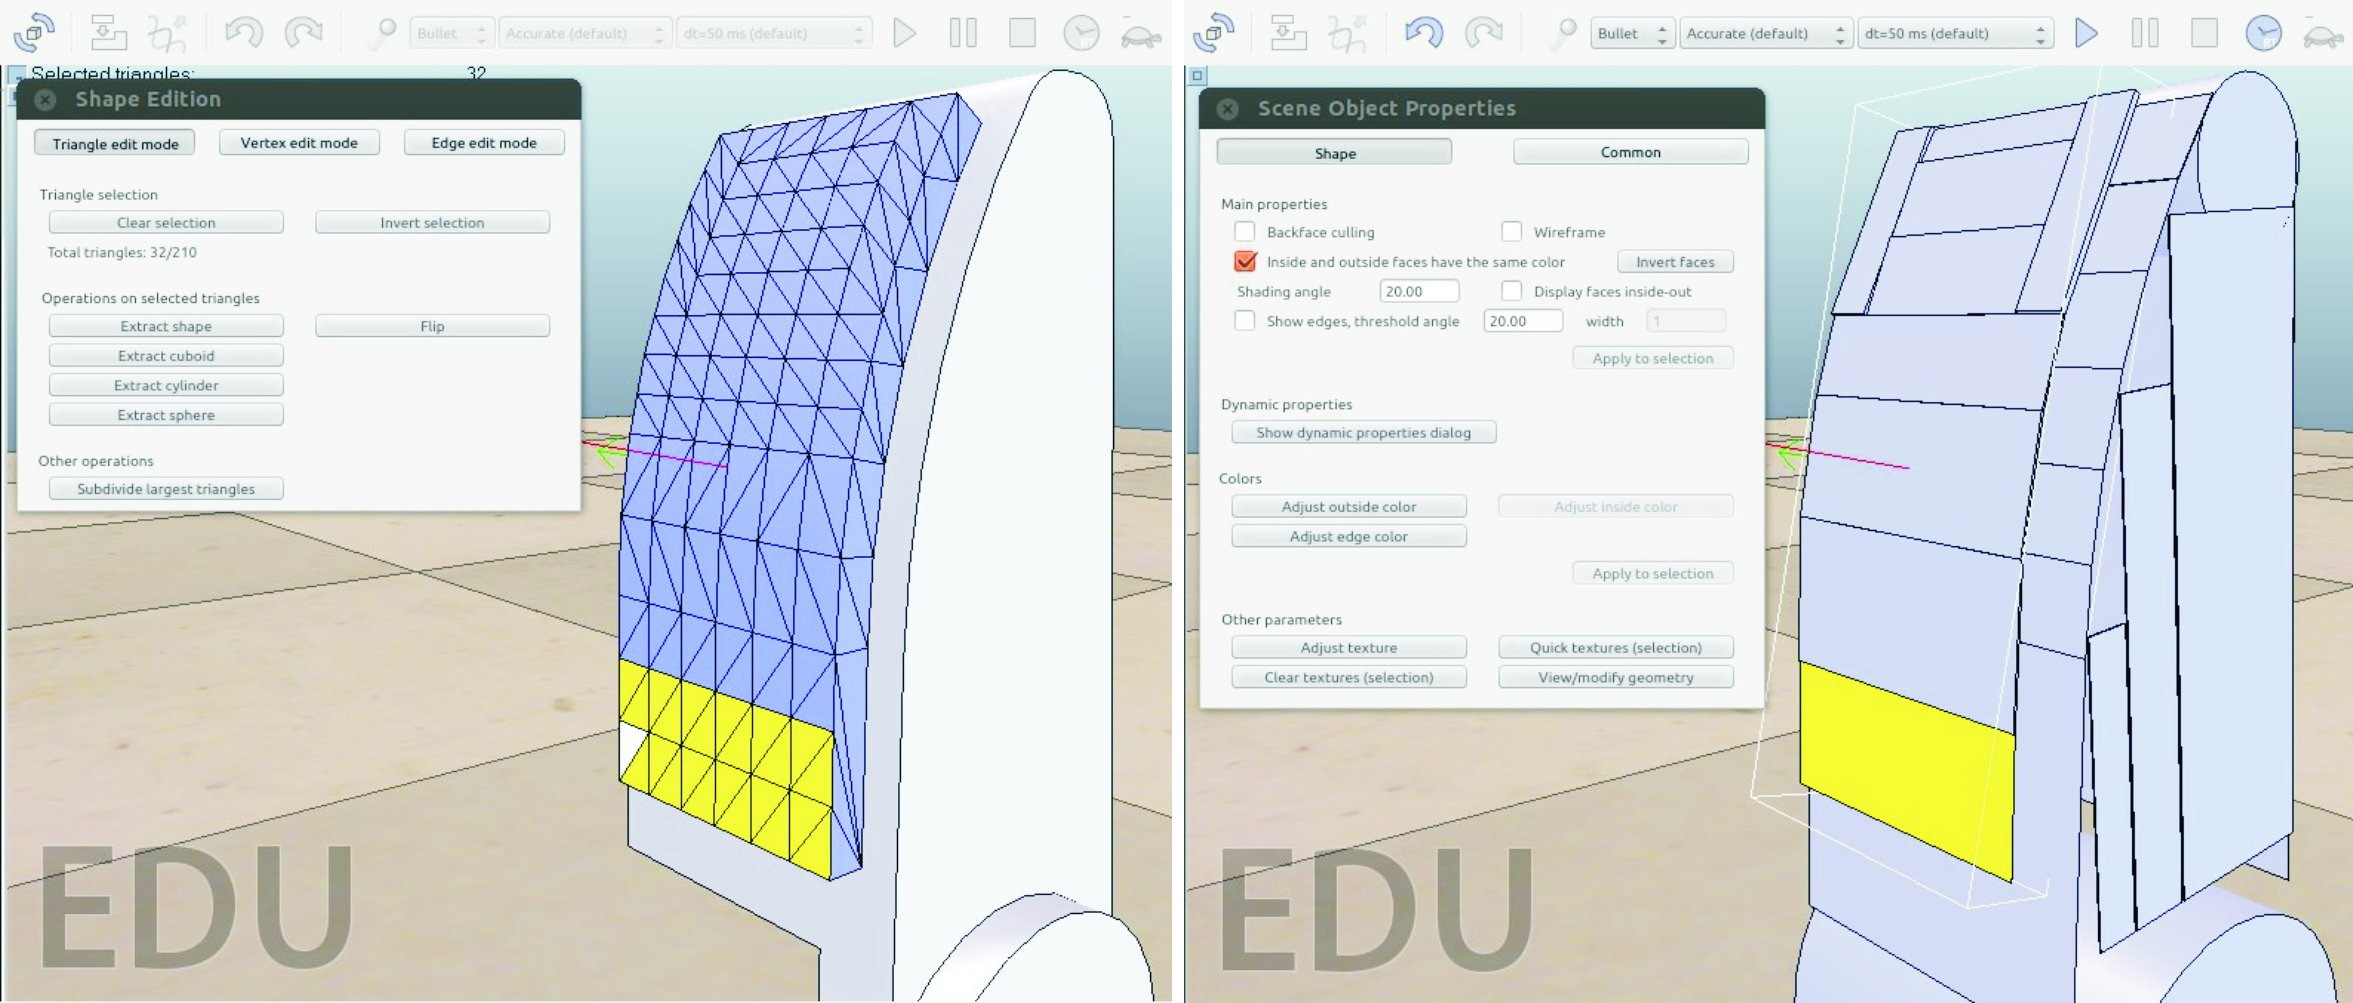
\includegraphics[width=1.0\textwidth]{images/extract_pure_shapes.jpg}
	\caption{Process of approximating the original mesh with pure shapes}
	\label{fig:ex_pure_shape}
\end{figure}
The extraction process is visualized in Figure\ref{fig:ex_pure_shape}. Dynamic parameters like mass and inertial matrix have been provided by Alex Rietzler. The predefined \emph{highFrictionMaterial} setting was used for each single part of the finger because that showed better results when picking up objects later on.\\

The last step of the modelling process was the adjustment of the model hierarchy. Root element of the hand model is the respondable part of the wrist which is also the dedicated model base. It is very important to follow the V-Rep guidelines for designing dynamic simulations because if the hierarchy is wrong, the model will simply fall apart when starting the simulation (detailed information can be found in the corresponding chapter\footnote{http://www.coppeliarobotics.com/helpFiles/en/designingDynamicSimulations.htm} of the V-Rep dodumentation). Each non-static and respondable shape has to be connected to it's parent by a joint or a force sensor. The visual part of the link is always a child object of it's corresponding respondable. That way, the kinematic chain of the gripper is formed.

\subsection{Assembling the scene}

\begin{figure}[ht]
	\centering
  	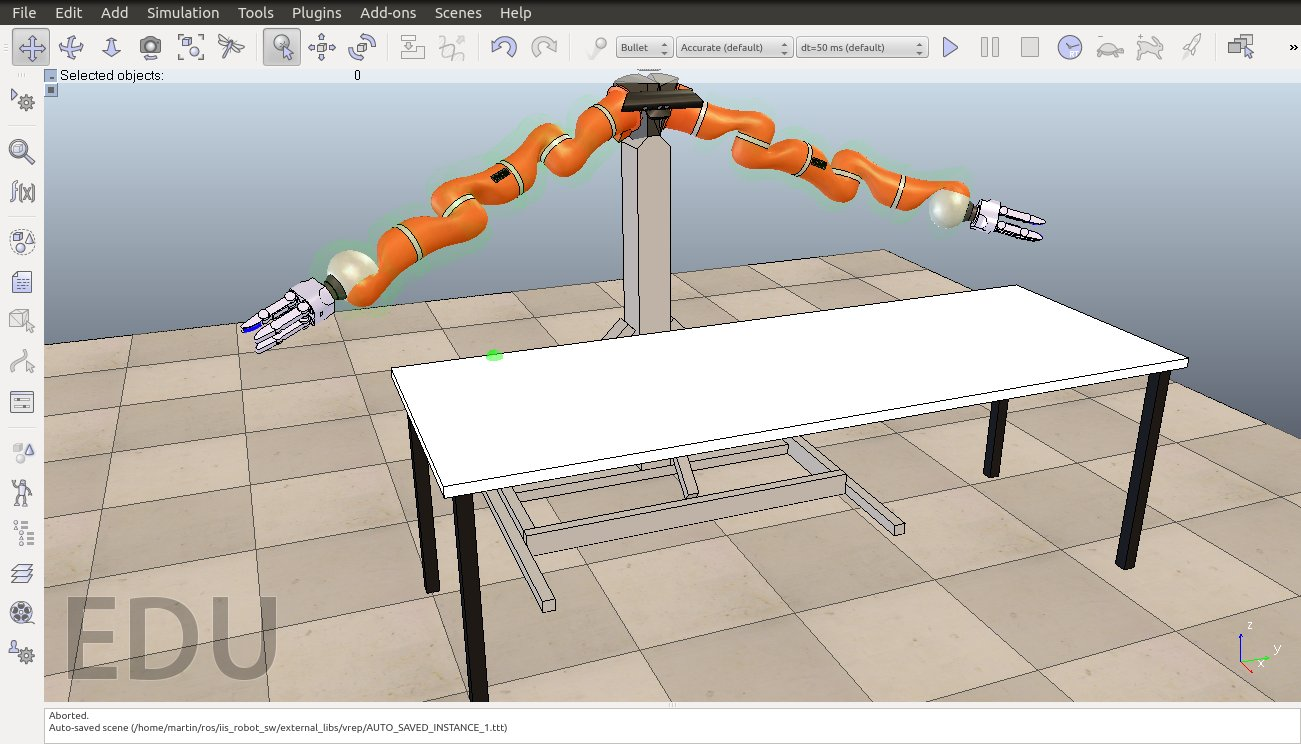
\includegraphics[width=1.0\textwidth]{images/simulation_scene.jpg}
	\caption{Structure of the V-Rep simulation scene}
	\label{fig:sim_scene}
\end{figure}

After finishing the gripper modelling process, each necessary component was available to build up the simulation scene as can be seen in Figure\ref{fig:sim_scene}. The final scene consists of a model of the robot's torso, two KUKA LWR4+ arm models with attached grippers and a model of the table in front of the robot. The origin of the world reference frame is located on the upper left side of the table, indicated by a slightly green shimmering sphere. A dummy object called \emph{ref\_frame\_origin} was placed at that location. Each position calculation later on will happen relative to that dummy element. If it is necessary to move the origin to another location within the workspace, this can simply be achieved by just moving that dummy to the required location. The position and orientation of the torso, the table and the two arms are set relative to the world reference frame. (TODO: transformation was provided - how was it achieved?). The grippers were placed on the tip of each arm. Within the scene hierarchy they are child elements of the last node in the corresponding arm tree. The correct rotation and offset was measured on the real counterpart and then adjusted accordingly. \\

The plate and the legs of the table were modelled as group of primitive cuboids. The table is defined as respondable to ensure that it will produce a collision reaction if a robot component collides with it. But as it is a static object it's position will not be influenced by such a collision because it is fixed within the scene. The material setting is set to \emph{highFrictionMaterial}. \\

The Kinect camera model was also taken from the model browser. As it's position and orientation in the real world is not fixed and might change from time to time, it's position within the simulation scene is just an approximation to reflect the real world setting as good as possible. 

\subsection{Configuring the collision detection module}

One of the requirements to the final solution is the ability to detect and visualize possible accidental collisions of the simulated robot with itself or it's environment. Moreover it would be a convenient feature to have some kind of warning if some of the robot's parts come dangerously close to an obstacle during movement. This could be achieved by creating a \emph{collision shield}, which means an enlarged version of the robot and do additional collision checking. These considerations lead to two different types of possible collisions. \emph{Soft collisions} are collisions, detected on the collision shield of the model. They just indicate a warning that the robot comes very close to an object it is not allowed to touch. \emph{Hard collisions} mean that a robot component directly hits another collidable object. This would be also a collision in the real world. The solution should be able to distinguish cleanly between those two types.\\ 

\begin{figure}[hb]
	\centering
  	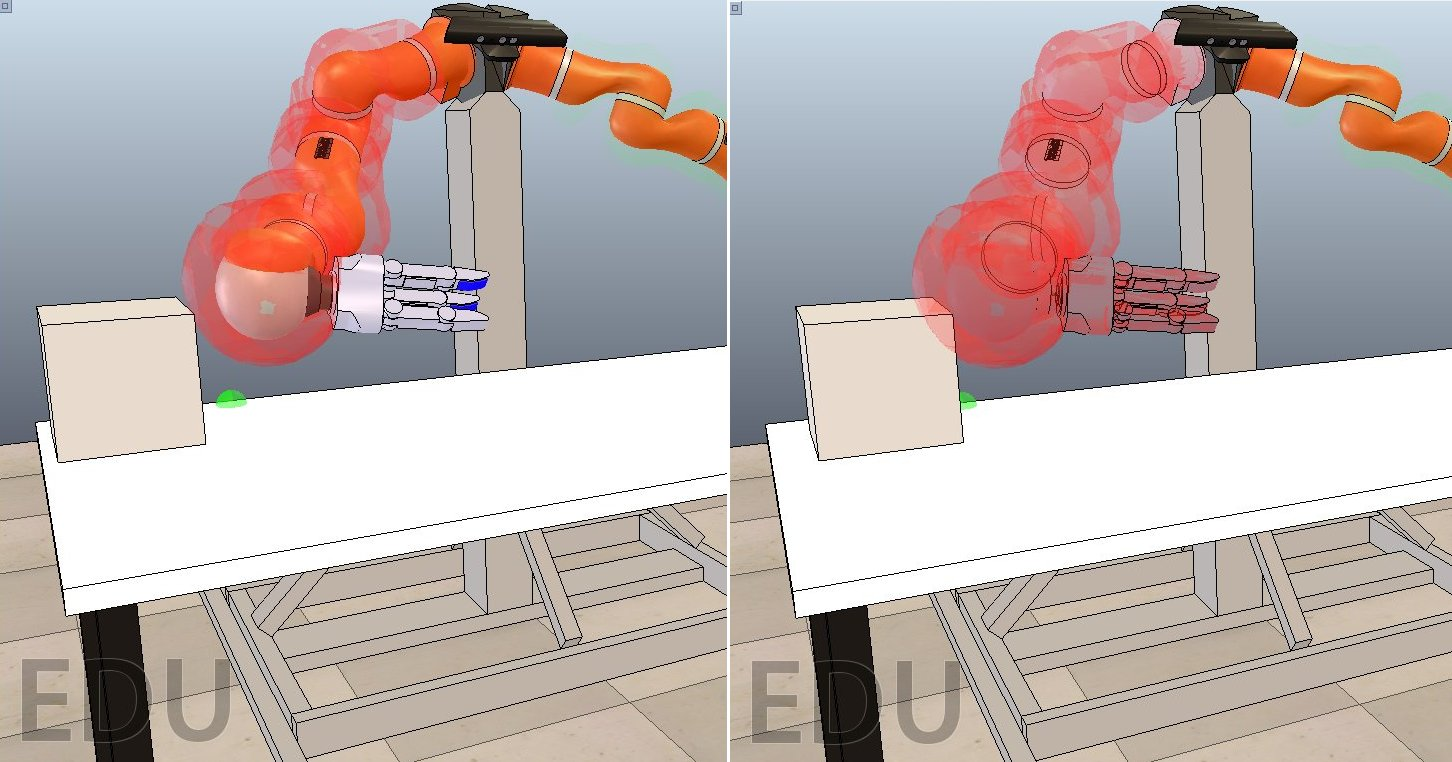
\includegraphics[width=1.0\textwidth]{images/collision.jpg}
	\caption{Collision detection and visualizing. The left image shows a hit on the collision shield, the right image indicates a direct hit.}
	\label{fig:collision}
\end{figure}

That goal was achieved by using V-Rep's \emph{collision detection module}\footnote{http://www.coppeliarobotics.com/helpFiles/en/collisionDetection.htm}. This calculation module is capable of detecting and visualizing collisions within the simulation scene by checking for interferences between \emph{collidable} shapes. It is important to understand that the collision detection module only \textit{detects} collisions. Producing \emph{collision reactions} is the responsibility of the \emph{dynamics module} and the chosen physics engine. Usually the shapes that form the visual part of the model are used for collision checking. The configuration is done by registering one or more \emph{collision objects}. Each collision object consists of a \emph{collider} and a \emph{collidee}. Both of them can be single shapes or collections of shapes. The collidee settings also offer the option \emph{all other collidable objects in the scene}. In that case, the collider is checked against all elements in $S=\{~s~|~s\in\textit{scene and}~s\notin\textit{collider}~\}$. The big advantage in using collections is that they allow to exactly describe which shapes should be checked against which other ones. Detected collisions are visualized by applying different colouring either to the collider or to the collidee as can be seen inf Figure\ref{fig:collision}. \\

The first step during realization was to model the collision shield. Therefore it was necessary to create an additional shape for each link that is slightly larger than the original one. This modelling process started at the second link of each robot arm and for all subsequent links the following steps were performed:

\begin{itemize}

\item
Create a copy of the shape that forms the visible part of the robot link
\item
Morph the copied object into a group of convex shapes to reduce complexity. This can be done by using the corresponding shape editor functionality.
\item
Ungroup the resulting group of shapes and merge them into one single shape
\item
Grow the resulting shape, but only in x and y direction of it's own reference frame. The resulting mesh should be approximately 10cm larger but keep the same height.
\item
Adjust the outside color to make it green and nearly transparent. The collision shield should be visible but not occlude the original model.
\item
Apply a meaningful name to the newly created shape to be be able to easily identify it within the model hierarchy. Here the name of the original shape with the '\_col' suffix was used.
\item
Make the new shape a sibling of the original one within the model hierarchy.
\item
Adjust the shape object properties. Define the new shape to be \emph{static} and \emph{non-respondable}.
\item
Disable the \emph{collidable} flag on the shape. This behaviour will be overridden in the collection
settings later on when configuring the collision detection module.

\end{itemize}

This modelling process is visualized in Fig???.\\

The next step was to adjust the configuration of the \emph{collision detection module}. Each arm requires two \emph{collision objects}, defined as stated in Figure\ref{fig:col_groups}. 
\begin{table}
  \centering
  \label{fig:col_groups}
  \begin{tabular}[h]{|l|l|l|} \hline
	\textbf{Collision object} & \textbf{Collider} & \textbf{Collidee} \\ \hline
	left\_arm & leftArm & all other entities \\
	right\_arm & rightArm & all other entities \\
	left\_armShield & leftArmShield & exLeftArmShield \\
	right\_armShield & rightArmShield & exRightArmShield \\ \hline
  \end{tabular}
  \caption{Configured collision objects}
\end{table}
The first two collision objects are designed to detect direct hits on the corresponding arm.  
Therefore the colliders (collections \emph{leftArm} and \emph{rightArm}) are checked for collisions against \emph{all other collidable objects in the scene}. This setting is only possible because the \emph{collidable} flag is disabled within the scene object settings of the collision shield elements, which means that they are excluded from collision checking by default. The collision objects, named with the \emph{Shield} suffix are responsible to check for hits solely on the collision shield elements. The colliders (collections \emph{leftArmShield} and \emph{rightArmShield}) consist only of the collision shield elements. As those elements were defined without the \emph{collidable} flag, the option \emph{Collection overrides collidable properties} is selected in the corresponding settings to explicitly enforce collision checking when using those collections. The collections, defining the collidees (\emph{exLeftArmShield} and \emph{exRightArmShield}) include all other objects except those, contained in the left/right arm's subtree. This exclusion is necessary because otherwise those collision objects would detect collisions between the shield elements and the other arm links. The collection definitions can be seen in Figure\ref{fig:col_defs}.
\begin{table}
  \centering
  \label{fig:col_defs}
  \begin{tabular}[h]{|l|l|} \hline
	\textbf{Collection} & \textbf{Definition} \\ \hline
	leftArm & $\{~s~|~s\in\textit{subtree of left arm}~\}$ \\
	leftArmShield & $\{~t~|~t\in\textit{element of left collision shield}~\}$ \\
	exLeftArmShield & $\{~u~|~u\in\textit{scene and}~u~\notin\textit{subtree of left arm}~\}$ \\
	rightArm & $\{~v~|~v\in\textit{subtree of left arm}~\}$ \\
	rightArmShield & $\{~w~|~w\in\textit{element of left collision shield}~\}$ \\
	exRightArmShield & $\{~x~|~x\in\textit{scene and}~x~\notin\textit{subtree of right arm}~\}$ \\ \hline
  \end{tabular}
  \caption{Collection definitions}
\end{table}
All collision objects are defined not to be handled explicitly. This means that V-Rep does not check them automatically on each simulation pass. It has to be done manually and will be explained later on in the section about control interface implementation.

\subsection{Configuring the IK calculation module}

The ROS control interface needs the ability to set arm target positions in \emph{joint space} or in \emph{Cartesian space}, depending on the selected control mode. Joint space targets are relatively easy to handle as that only means to set the target position of each single joint. Setting targets in Cartesian space requires to solve the inverse kinematics problem for the corresponding robot component. Therefore V-Rep offers the \emph{inverse kinematics calculation module} \footnote{http://www.coppeliarobotics.com/helpFiles/en/inverseKinematicsModule.htm}. 
This calculation module allows to define and register various \emph{IK groups}. Each IK group has to contain at least one \emph{IK element}, defining the kinematic chain, constraints and desired precision settings (linear and angular). IK elements can be configured to enforce position constraints and/or orientation constraints for each single axis. The kinematic chain is specified by selecting the dedicated base link and the tip. The tip is a dummy object, indicating the end effector reference frame. The IK target is defined by another dummy object. Tip and target have to be linked, forming a \emph{IK, tip-target} connection by selecting the appropriate link type within the dummy object settings. Figure\ref{fig:ik_vrep} shows a schematic description of that concept. The target pose is set by placing the target dummy at the desired location. The IK calculation model will then adjust the joint positions until the tip pose matches the target pose, respecting joint limits and configured constraints and tolerance values. The joints within the specified kinematic chain need to be operated in \emph{inverse kinematics mode}, otherwise the module is not able to control them.

\begin{figure}[ht]
	\centering
  	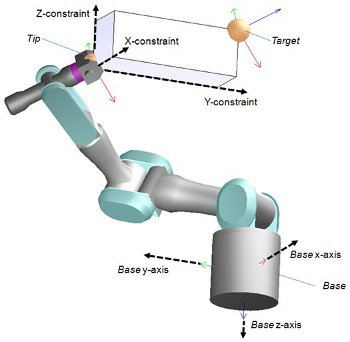
\includegraphics[width=0.5\textwidth]{images/ik_vrep.jpg}
	\caption{IK calculation module concept}
	\label{fig:ik_vrep}
\end{figure}

The IK calculation module allows to define various IK groups for each robot component with differing configurations. Along the collection of IK elements, the IK group settings include the desired calculation method and the maximum amount of calculation iterations to use. Available IK calculation methods are \emph{pseudo inverse} (PI) and \emph{damped least squares} (DLS). As stated by \cite{buss2004}, the PI method is usually faster than DLS. The tradeoff is that PI tends to be unstable in configurations where the target position is unreachable. That fact leads to a jittery behaviour of the manipulator. The DLS method provides higher stability in such situations but requires more calculation time.

\begin{table}[h]
  \centering
  \label{fig:ik_defs}
  \begin{tabular}[h]{|l|c|c|c|} \hline
	\textbf{IK group} & \textbf{Method} & \textbf{Iterations} & \textbf{Prec. lin/ang} \\ \hline
	left\_arm & PI & 9 & 0.001 / 0.1  \\
	left\_arm1 & PI & 3 & 0.002 / 0.2  \\
	left\_arm2 & DLS & 3 & 0.002 / 0.1  \\
	right\_arm & PI & 9 & 0.001 / 0.1  \\
	right\_arm1 & PI & 3 & 0.002 / 0.2  \\
	right\_arm2 & DLS & 3 & 0.002 / 0.1  \\ \hline
  \end{tabular}
  \caption{IK group definitions}
\end{table}

Three IK groups have been created for each arm. The configuration settings are listed in Figure\ref{fig:ik_defs}. They were chosen, following the guidelines from the V-Rep documentation. The first two groups use the faster PI calculation method. The first one allows a higher amount of maximum iterations while demanding stricter precision settings than the second one. The third one is designed to increase stability especially for positions close to singularities. Therefore the DLS method was chosen with an increased position tolerance value. That configuration is less performant because of the DSL calculation method and therefore it is only used if the other groups failed to find a solution. The IK groups are called sequentially until one of them is able to solve the problem. This process is explained in the ROS control interface section later on.

\section{Implementing the ROS control interface}

In the real world, each type of robot component has its own, clearly defined ROS control interface. Those interfaces are composed from sets of inbound and outbound ROS topics that allow sending commands and to retrieve state data. The simulated components have to provide exactly the same ROS interface as their real counterparts, using similar topic names and message types. The structure of this control flow can be seen in Figure\ref{fig:control_flow}.

\begin{figure}[ht]
	\centering
  	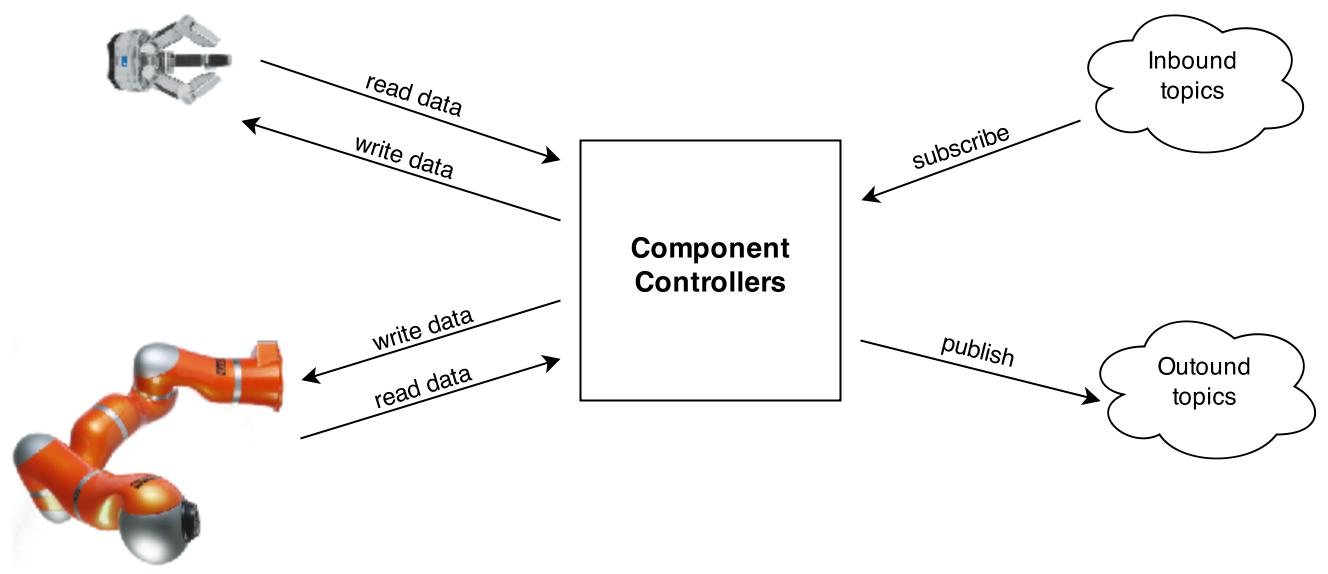
\includegraphics[width=1.0\textwidth]{images/control_flow.jpg}
	\caption{Control flow structure}
	\label{fig:control_flow}
\end{figure}

The existing ROS interface that is part of the V-Rep distribution is not suitable as it only provides a very general approach for controlling joint values and reading state data. Therefore V-Rep provides various extension points, allowing to add custom functionality. The final solution was implemented as a \emph{simulator plugin}, written in C++ and using V-Rep's \emph{regular API}\footnote{http://www.coppeliarobotics.com/helpFiles/en/apiOverview.htm}. This approach states the most flexible solution as this API provides more than 400 functions that can be used to extend the simulator functionality. A plugin is a compiled library file, written in C++ that has to follow some V-Rep specific naming conventions and must reside in the V-Rep working directory. The library file gets automatically loaded on V-Rep startup and runs in the main simulation thread. The source code is located in the \emph{iis\_simulation} package that is part of the \emph{iis\_robot\_sw} repository. The following section describes the design of the plugin architecture and the most important components within the package.

%The first problem that arose when starting the implementation process was, how each type of robot component can be clearly identified within a simulation scene. V-Rep is a simulation environment that allows to load and simulate multiple scenes. A scene is a hierarchy of various scene objects, organized in a tree structure and those objects can be shapes, joints, sensors or even only dummies. The scene content can be modified by the user. Arbitrary objects can be added or removed, maybe a gripper gets replaced by another component, an arm gets removed or an additional Kinect camera gets installed. The required solution should be able to react to those changes. Parts of the hierarchy should be clearly identifiable as a specific simulation component. Each single part of a component should be identifiable (joints, sensors, dummies, IK groups, collision objects). Luckily V-Rep provides various extension points for programmers and is therefore highly customizable. 

%\begin{figure}[ht]
%	\centering
%  	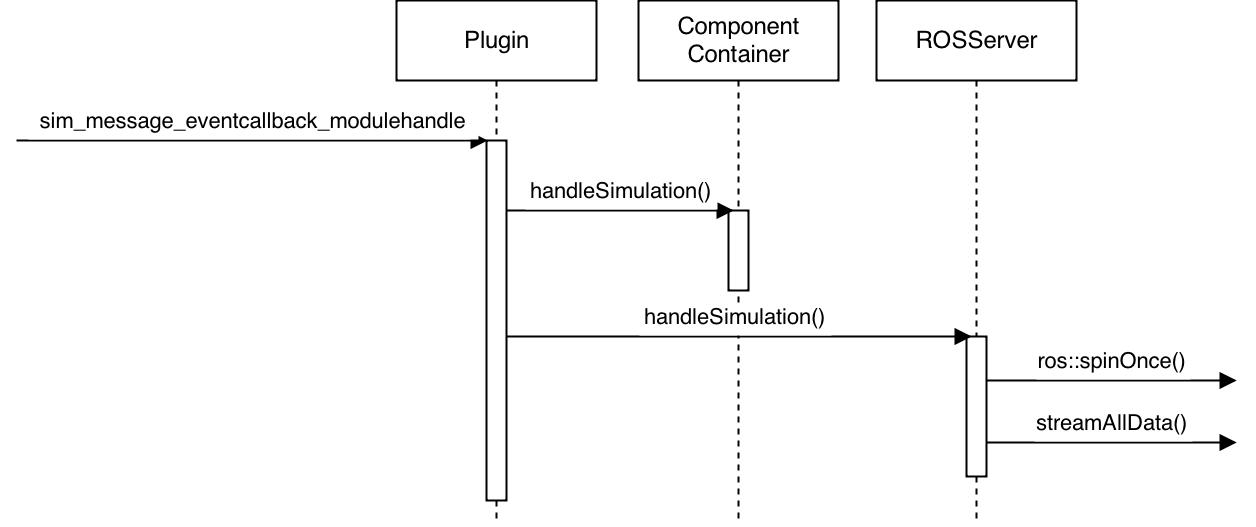
\includegraphics[width=1.0\textwidth]{images/handle_sim.jpg}
%	\caption{Handling a simulation step}
%	\label{fig:handle_sim}
%\end{figure}

\subsection{Plugin architecture}

A plugin is a compiled library file, written in C++. This library needs to be placed in the V-Rep working directory and follow the V-Rep specific naming conventions. On startup, V-Rep looks for library files, prefixed with 'libv\_repExt'. Matching files are automatically loaded. A plugin runs in the main simulation thread -  that means it has to be programmed really carefully to avoid performance leaks during simulation. The plugin has to provide a clearly defined interface, consisting of 3 function definitions:

\begin{itemize}

\item \texttt{unsigned char v\_repStart(void* reserved,int reservedInt)} \\
This function is called on V-Rep startup and is used to perform necessary initialization steps. A return value of zero indicates that the initialization process failed and the plugin gets unloaded immediately. The current solution depends on a running roscore during startup. If that is not the case it is not able to work.

\item \texttt{void v\_repEnd()} \\
Called before shutdown and is used to do some general cleanup and free allocated memory.

\item \texttt{void* v\_repMessage(int msg, int* auxData, void* custData, int* resData)} \\
This function is called very often during the whole V-Rep lifecycle and is therefore a very performance critical method. Via this function V-Rep notifies plugins about events like start/end of simulation, simulation step, scene content change, scene switch and more. The plugin code can react to those events accordingly. In the current implementation, those messages are just passed to the software components that are responsible to handle the specific action. 
  
\end{itemize}

The plugin code is organized as can be seen in the UML diagram in Figure\ref{fig:plugin_uml}. The major parts of the system are described in the subsequent paragraphs.

\paragraph{SimulationComponent}

A simulation component is a single, reusable model of a specific robot component that can be utilized in different environments. Each component provides it's own clearly defined control interface. A simulation scene can contain multiple components from various types. The \emph{SimulationComponent} class is the abstract base class for all simulation components. Currently there are existing two concrete implementations -- the \emph{LWRArmComponent} and the \emph{SchunkHandComponent}. If the scenario should be extended and new components have to be introduced, it is necessary to create a new subclass of \emph{SimulationComponent} and provide implementations for the abstract methods. 

\begin{figure}[t]
	\centering
  	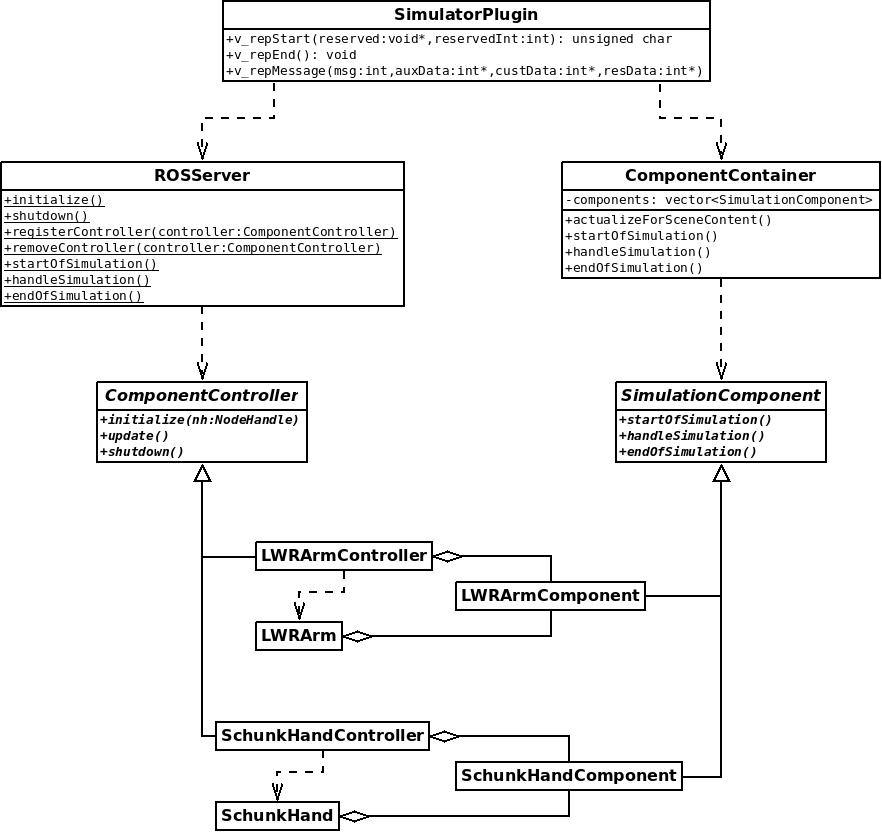
\includegraphics[width=1.0\textwidth]{images/SimulatorPluginUML.jpg}
	\caption{Simulator plugin architecture}
	\label{fig:plugin_uml}
\end{figure}

\paragraph{ComponentContainer}

This class represents the set of all identified simulation components within the current scene. On V-Rep startup an instance of \emph{ComponentContainer} is created. Each time, the content of the current simulation scene changes, the method \emph{actualizeForSceneContent} is triggered. This method then performs the following steps:
\begin{itemize}

\item
It validates all currently registered \emph{SimulationComponent} instances if they are still valid and present in the scene.
\item
It traverses the whole scene hierarchy to identify newly created components
\item
If a new component is identified, a corresponding concrete instance of \emph{SimulationComponent} is created and added to the container.

\end{itemize}
  
The process of traversing the scene hierarchy and identifying components is explained in section\ref{sec:comp_id}. During a running simulation, the \emph{ComponentContainer} gets notified about each single simulation step. It simply forwards that message to all registered components. Those can then perform all necessary steps like triggering collision checking or handling IK groups.
  
\paragraph{ROSServer}

The \emph{ROSServer} is a static class that encapsulates all ROS related functionality. It tries to initialize ROS on plugin startup, forcing a shutdown, if the connection to the master cannot be established. Otherwise it creates and maintains a ROS \emph{NodeHandle} for the 'simulation' namespace. Each \emph{SimulationComponent} can register \emph{ComponentController} instances at the \emph{ROSServer}. On simulation start it initializes all registered controllers with the maintained \emph{NodeHandle}. The \emph{ROSServer} gets also notified about each simulation step and forces the controllers to handle the received commands and publish all the necessary data. On simulation end it triggers the shutdown of all registered controllers.
  
\paragraph{ComponentController}

This is the abstract base class for all controllers. A controller actually represents the ROS interface of a specific simulation component, maintaining all the inbound and outbound topics used to control the simulated hardware. It is responsible for delegating commanded values to the underlying component as well as reading and publishing state data. Concrete implementations are the \emph{LWRArmController} and the \emph{SchunkHandController}. A \emph{ComponentController} needs to be registered at the \emph{ROSServer} and gets initialized on simulation start. Concrete implementations can use the provided NodeHandle to create all the necessary publishers and subscribers. The \emph{update} method is called by the \emph{ROSServer} on each simulation step and forces the controller to publish all the required data. The \emph{shutdown} method is called by the \emph{ROSServer} on simulation end, forcing the controller to shutdown all publishers and subscribers. \\

\subsection{Identifying simulation components}
\label{sec:comp_id}

The plugin functionality should not be tied to a specific simulation scene but to specific models of robot components. Each time a known component is added to the scene it should be recognized by the plugin and the corresponding instance of \emph{SimulationComponent} has to be instantiated and added to the \emph{ComponentContainer}. As visualized in Figure\ref{fig:scene_tree}, each simulation scene
is a tree structure, consisting of various different types of scene objects. 
\begin{figure}[h]
	\centering
  	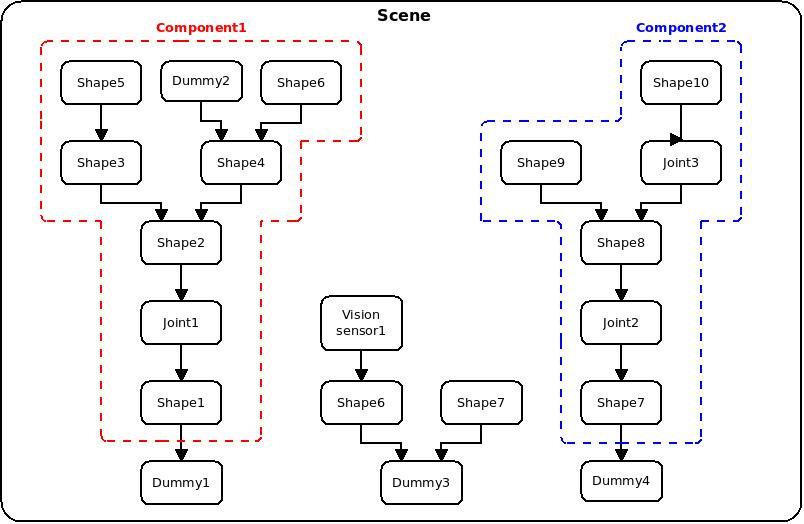
\includegraphics[width=0.8\textwidth]{images/scene_hierarchy.jpg}
	\caption{Sample scene hierarchy}
	\label{fig:scene_tree}
\end{figure}
It is necessary to identify subtrees within this hierarchy that belong to known simulation components and should therefore be handeled by the plugin. If a component is identified, the plugin has to discover each single part of the model. Depending on the model this can be joints, force sensors, reference frame dummies, IK groups or collision objects.

One possible way would be to give each part a clearly defined, unique name and then search for those names within the scene. But this approach would require to hardcode each single object identifier and this is not a preferable solution for this problem. If a user accidentally changes a name inside the model tree then the solution is broken because the plugin looses connection to the underlying object and cannot control it any more. Here V-Rep's custom developer data functionality comes into play. It is possible to put auxiliary data segments to each single object in the scene. Those data segments are serialized together with the object and can be read programatically. Each data segment starts with a header number which is used to uniquely identify the data from a specific developer. A visualization of this concept can be seen in Figure\ref{fig:cust_dev_data}. 
\begin{figure}[h]
	\centering
  	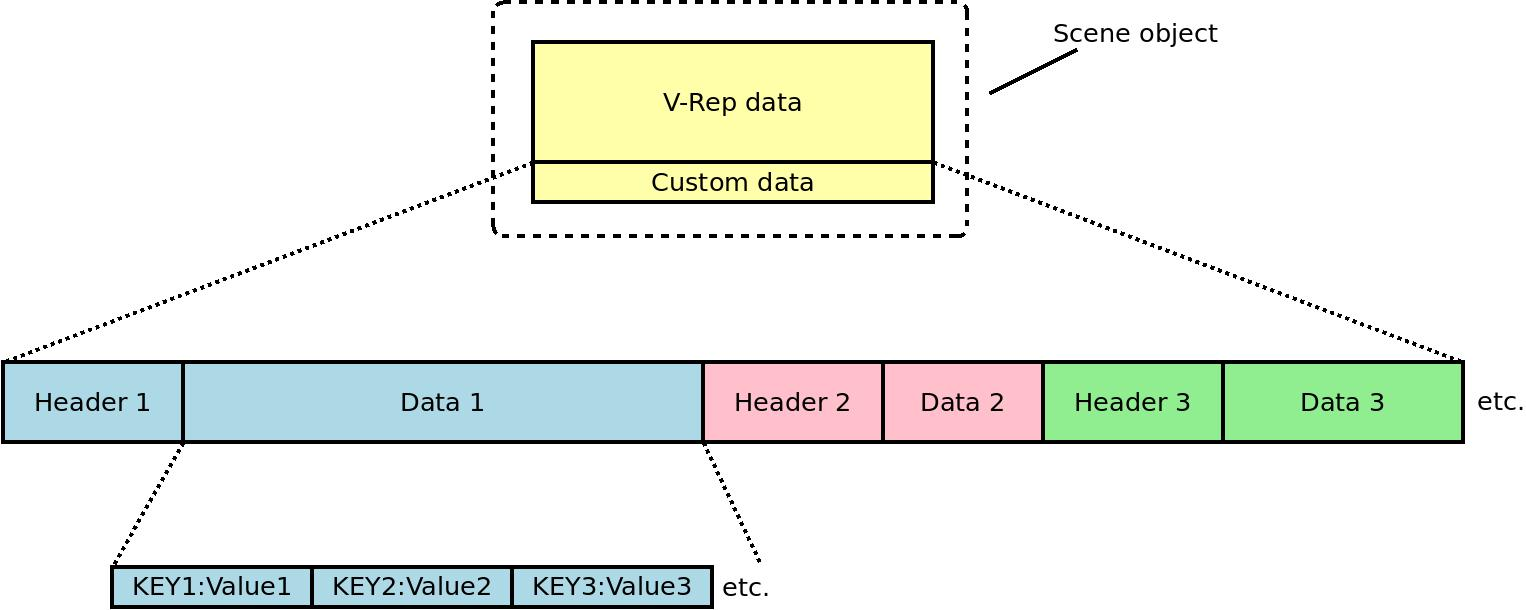
\includegraphics[width=1.0\textwidth]{images/custom_dev_data.jpg}
	\caption{Custom developer data segments on scene object}
	\label{fig:cust_dev_data}
\end{figure}

As the format of the data can freely be chosen, it was decided to use string representations of key/value pairs, separated by a colon (:). The key is an integer number, used to determine the type of the tagged object. The value segment can be used to provide additional information, e.g. the name of a joint. The left arm's model base for example is tagged with the data segment \texttt{2497,1:left\_arm}. The number 2497 is the header that identifies the data segment to belong to this plugin. The data segment identifies that element as the model base of a \emph{LWRArmComponent} (Key=1) with the name \emph{left\_arm}. The available keys are explained in the sections that correspond to the specific simulation components.

When actualizing for scene content change, the \emph{ComponentContainer} traverses the scene hierarchy and looks for objects, that are tagged as known components. On success, it creates the specific instance providing the object ID of the underlying scene object to the constructor. During initialization, the concrete \emph{SimulationComponent} implementation then traverses the rest of the model subtree to extract all the remaining parts that belong to that specific model (joints, dummies, force sensors...), also by looking for tagged objects. The implementations for arm and hand model provide feedback output on the console window about the status of this initialization process and provide meaningful error messages in case that not all necessary parts of a model could be successfully located.

\subsection{The LWRArmComponent}

The \emph{LWRArmComponent} is a concrete subclass of \emph{SimulationComponent} and states the abstraction of a simulated KUKA LWR4+ arm model. It is composed of two parts - an instance of the \emph{LWRArm} class and a corresponding \emph{LWRArmController}, as can be seen in the UML diagram in Figure\ref{fig:plugin_uml}. Their functionalities are explained in the following paragraphs.

\paragraph{LWRArm}

This class states the connection to the (simulated) hardware itself, providing methods to set commanded values and access all available state data like joint positions, Cartesian position of the end effector, current collision state and more. On creation, it is passed the base of the model tree as constructor argument. The base is identified by the LWR\_ARM\_COMPONENT tag. The value segment of this tag states the name of the arm which has to be unique within the scene. During initialization it traverses the model tree and extracts all required parts by searching for tagged scene objects as described in the previous chapter. The parts to identify are the 7 arm joints, the force sensor on the last link of the arm, IK tip and target dummies. The corresponding tags are listed in Table\ref{fig:lwr_tags}.
\begin{table}[ht]
  \centering
  \label{fig:lwr_tags}
  \begin{tabularx}{\textwidth}{|l|l|l|X|} \hline
	\textbf{Constant} & \textbf{Key} & \textbf{Value} & \textbf{Description} \\ \hline
	LWR\_ARM\_COMPONENT & 1 & Arm name & Identifies KUKA LWR arm model \\
	LWR\_ARM\_JOINT & 12 & Joint name & Joint in KUKA LWR arm \\
	LWR\_ARM\_CONNECTOR & 13 & - & Force sensor on arm tip \\
	LWR\_ARM\_TIP & 14 & - & IK tip dummy \\
	LWR\_ARM\_TARGET & 15 & - & IK target dummy  \\ \hline
  \end{tabularx}
  \caption{Tag data items for LWRArmComponent}
\end{table}
Additionally the \emph{LWRArm} also requires a connection to the configured IK groups and collision objects. As there is no possibility to place custom developer tags on IK groups and collision objects, the extraction is done by using a special naming strategy. The first IK group needs to have the same name as the arm itself and it's existence is mandatory, leading to a configuration error message if no such group can be extracted during initialization. Subsequent groups are optional and must have the same name with consecutive numbering (ARM\_NAME1, ARM\_NAME2, \ldots). That allows to reconfigure the IK calculation module and introduce additional IK groups without touching the plugin code. The two required collision objects are also searched, based on the name of the arm (ARM\_NAME and ARM\_NAMEShield). If one or both of them cannot be detected, an error message is stated on the console and the collision detection functionality will not work as expected.

To fullfill the requirements for the control interface, the arm has to be able to operate in joint control mode (FK mode) and in inverse kinematics mode (IK mode). Initially the arm starts in FK mode, which means the joints are operated in \emph{torque/force} mode and accept target positions to be set. Switching to IK mode is done by changing the joint control mode to \emph{inverse kinematics} mode, which means that they are conntrolled by the IK calculation module further on. Setting a target pose in Cartesian space is done by moving the IK target dummy to the required location and orientation. The known IK groups are then handled sequentially, until one of them is able to solve the problem and set the proper joint target positions. When switching from FK to IK mode, the IK target dummy has to be aligned with the tip dummy to prevent the arm from doing uncontrolled motions.

The current collision status is determined by using the configured collision objects. On each simulation step the collision object that is responsible for detecting direct collisions is handled first. If that one detects a collision, a direct hit is reported and it is not necessary to handle the second object at all, because a direct hit always implies a hit with the shield as well. Only if no direct hit was detected, the second collision object is handled. The outcome can be queried as the current collision state of the arm. The collision state is evaluated on each simulation step.

\paragraph{LWRArmController}

The \emph{LWRArmController} is a subclass of \emph{ComponentController} that encapsulates the whole ROS interface to the \emph{LWRArmComponnt}. On creation it is passed a reference to the underlying \emph{LWRArm}. The arm controller offers 3 basic control modes:

\begin{itemize}

\item \textbf{Joint control mode} \\
The controller accepts target positions in joint space via the \texttt{joint\_control/move} topic. The message basically consists of a vector, containing a target angles for each single joint, measured in \emph{radiant}. Incoming target positions are validated not to exceed a specified velocity limit, enforcing the constraint
\begin{equation}
  |c_{i}-t_{i}|<\delta, \forall ~i~\in~[0,6]
\end{equation}
where $c_{i}$ are current and $t_{i}$ are target positions for the joints 0 to 6 and $\delta$ is the current velocity limit. If the velocity limit is violated, the message is dropped and a corresponding error message is published to the \texttt{sensoring/error} topic and written to the console output. The default limit is set to a value of 0.1 and can be adjusted via the \texttt{joint\_control/set\_velocity\_limit} topic. Valid target positions are simply passed to the underlying \emph{LWRArm} instance, which is operated in FK mode.

\item \textbf{Cartesian control mode} \\
The controller accepts target positions in Cartesian space via the \texttt{cartesian\_control/move} topic. Therefore, the \emph{LWRArm} needs to be operated in IK mode. The commanded target pose is also validated before accepting it. The constraint is defined as
\begin{equation}
  |c_{x}-t_{x}|<\sigma ~and~ |c_{y}-t_{y}|<\sigma ~and~ |c_{z}-t_{z}|<\sigma
\end{equation}
where $c$ is the current and $t$ is the target position in Cartesian space and $\sigma$ is the current Cartesian velocity limit. The velocity limit can be adjusted, using the \texttt{cartesian\_control/set\_velocity\_limit} topic. Invalid messages are dropped and result in an error message as well, published in \texttt{sensoring/error} topic. Valid target poses are passed to the underlying \emph{LWRArm}.

\item \textbf{Follow mode} \\
This mode is only on the simulator available and designed to mirror the behaviour of the real robot. The controller reads the joint states of it's real counterpart from the corresponding topic and uses it's current position as target. Therefore, the \emph{LWRArm} is operated in FK mode. This results in an exact copy of the real robot's motions. This mode can be used to test the accuracy of the simulated model, for example by carefully moving the robot close to positions where it collides with the table and check when the collision is reported. 

\end{itemize}

The controller has to be registered at the \emph{ROSServer} in order to be able to work. This section only covered the most important control modes and topics. The complete interface description can be found in the documentation, located in the appendix.

\subsection{The SchunkHandComponent}

The \emph{SchunkHandComponent} is designed, using the same approach as for the \emph{LWRArmComponent}. Therefore only the most important facts will be stated here. The two composing parts are the \emph{SchunkHand} and the \emph{SchunkHandController}.
\begin{table}[h]
  \centering
  \label{fig:schunk_tags}
  \begin{tabularx}{\textwidth}{|l|l|l|X|} \hline
	\textbf{Constant} & \textbf{Key} & \textbf{Value} & \textbf{Description} \\ \hline
	SCHUNK\_HAND\_COMPONENT & 2 & Hand name & Identifies Schunk hand model \\
	SCHUNK\_HAND\_JOINT & 22 & Joint name & Joint in Schunk hand model \\ \hline
  \end{tabularx}
  \caption{Tag data items for SchunkHandComponent}
\end{table}

\paragraph{SchunkHand}

States the connection to a Schunk hand model. The only additional parts that have to be discovered during initialization are the 7 gripper joints and their corresponding names. Available tags are
listed in Table\ref{fig:schunk_tags}. The \emph{SchunkHand} class provides methods to set joint positions and to retrieve current joint states. Additionally it allows to modify the motor strength for each single joint, based on a percentage of maximum force. This reflects the possibility of adjusting the motor currents in the real hand, which also leads to the effect that the maximum motor strengths of the finger joints can be increased or decreased.

\paragraph{SchunkHandController}

The \emph{SchunkHandController} provides an implementation of the ROS interface for the Schunk gripper model. The basic topics are quite similar to those of the \emph{LWRArmController}, as there are \texttt{joint\_control/move} for setting joint target positions or \texttt{joint\_control/get\_state} for retrieving joint states.
\begin{figure}[h]
	\centering
  	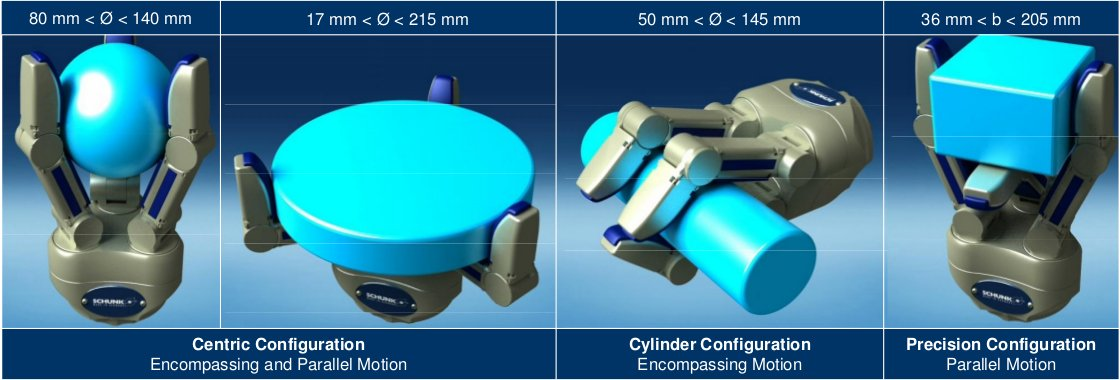
\includegraphics[width=1.0\textwidth]{images/grasp_types.jpg}
	\caption{Grasp types SPHERICAL, CENTRICAL, CYLINDRICAL and PARALLEL}
	\label{fig:grasp_types}
\end{figure}
Additionally the hand is able to perform grasps, based on specific \emph{grasp types} as can be seen in Figure\ref{fig:grasp_types}. This functionality can be accessed via the \texttt{joint\_control/gripHand} topic. A grasp is defined by the parameters \emph{grasp type} and \emph{close ratio}. The controller then calculates the corresponding joint positions, based on those parameters and sets the desired target positions. Each grasp can be expressed, using three functions -- one for the position of the pivoting joints and the other two for the positions of the distal and proximal finger joints. The utilized functions were taken from the original controller code of the \texttt{schunk\_sdh} ROS package, located in the \texttt{iis\_robot\_sw} code repository. The definitions can be seen in Table\ref{fig:grasp_defs}. The grasp strength can be adjusted, using the \texttt{settings/set\_motor\_current} topic. The message basically consists of a vector, holding a value for each joint, defining a percentage of the maximum motor strength. The real gripper also provides a topic that allows to read the current motor temperatures. For the sake of consistency, the \emph{SchunkHandController} also provides this topic, but as V-Rep is not able to simulate motor heatings, only constant fake values are published. A complete interface description can be found in the appendix.
\begin{table}[h]
  \centering
  \label{fig:grasp_defs}
  \begin{tabular}{|l|c|c|c|} \hline
	\textbf{Name} & \textbf{pivoting} & \textbf{proximal} & \textbf{distal} \\ \hline
	CYLINDRICAL & $0$ & $(-30+30x)\frac{\pi}{180}$ & $(30 + 35x)\frac{\pi}{180}$ \\
	PARALLEL & $0$ & $(-75+82x)\frac{\pi}{180}$ & $(75-82x)\frac{\pi}{180}$ \\
	CENTRICAL & $\frac{\pi}{3}$ & $(-75+82x)\frac{\pi}{180}$ & $(75-82x)\frac{\pi}{180}$ \\
	SPHERICAL & $\frac{\pi}{3}$ & $(-40+25x)\frac{\pi}{180}$ & $(40+15x)\frac{\pi}{180}$ \\ \hline
  \end{tabular}
  \caption{Joint position functions based on close ratio $x$}
\end{table}

\subsection{Publishing Kinect camera data}

The Kinect camera model does not contain any flexible parts that have to be controlled by the plugin. But it is necessary to make the images, captured by the simulated vision sensor available via ROS topics. This was achieved by using the corresponding functionality of the V-Rep default ROS interface that allows publishing vision sensor data, using the correct message types. Therefore a LUA script was attached to the base element of the camera model within the scene. This script simply extracts the object ID of the vision sensor and enables publishers for the captured RGB and depth images. The corresponding topics are \texttt{kinect1/sensoring/rgb\_image} and \texttt{kinect1/sensoring/depth\_image}. 
